\chapter{منحنيات شدة التيار--الجهد}\label{ch:b2:current-potential-curves}

يُطلى الفولاذ بالزنك كهربائيًا في أحواض حمضية. ومع ذلك يقول مخطط الجهد--pH
الوارد في مجلد السنة الأولى إن الزنك، الواقع بعيدًا تحت خط الهيدروجين، ينبغي أن يختزل
الحمض ويذوب بسرعة ترسبه نفسها. وهذا لا يحدث، لأن
المخطط يقول ما قد يحدث، لا بأي سرعة. فسرعة تفاعل القطب
تيار، ورسم هذا التيار بدلالة جهد القطب
يُظهر فورًا أي التفاعلات سريعة، وأيها بطيئة، وأيها يحدّها
وصول المتفاعل. ومنحنيات شدة التيار--الجهد هذه هي أداة
كل كيميائي كهربائي يطلي فلزًا، أو يشحن بطارية، أو يقيس
الأكسجين في نهر.

\begin{recall}
مجلد السنة الأولى: جهد القطب، والقطب المرجعي، ومعادلة
نرنست، ومخططات الجهد--pH وحدّها (تقول ما هو ممكن، لا بأي
سرعة). \Cref{ch:b2:cell-thermodynamics}: $\Delta_r G = -nFE$، ومعادلة نرنست
مبرهنةً. ومن الفيزياء: الانتشار وقانون فيك، $j = -D\,dc/dx$.
\end{recall}

\begin{omfigure}
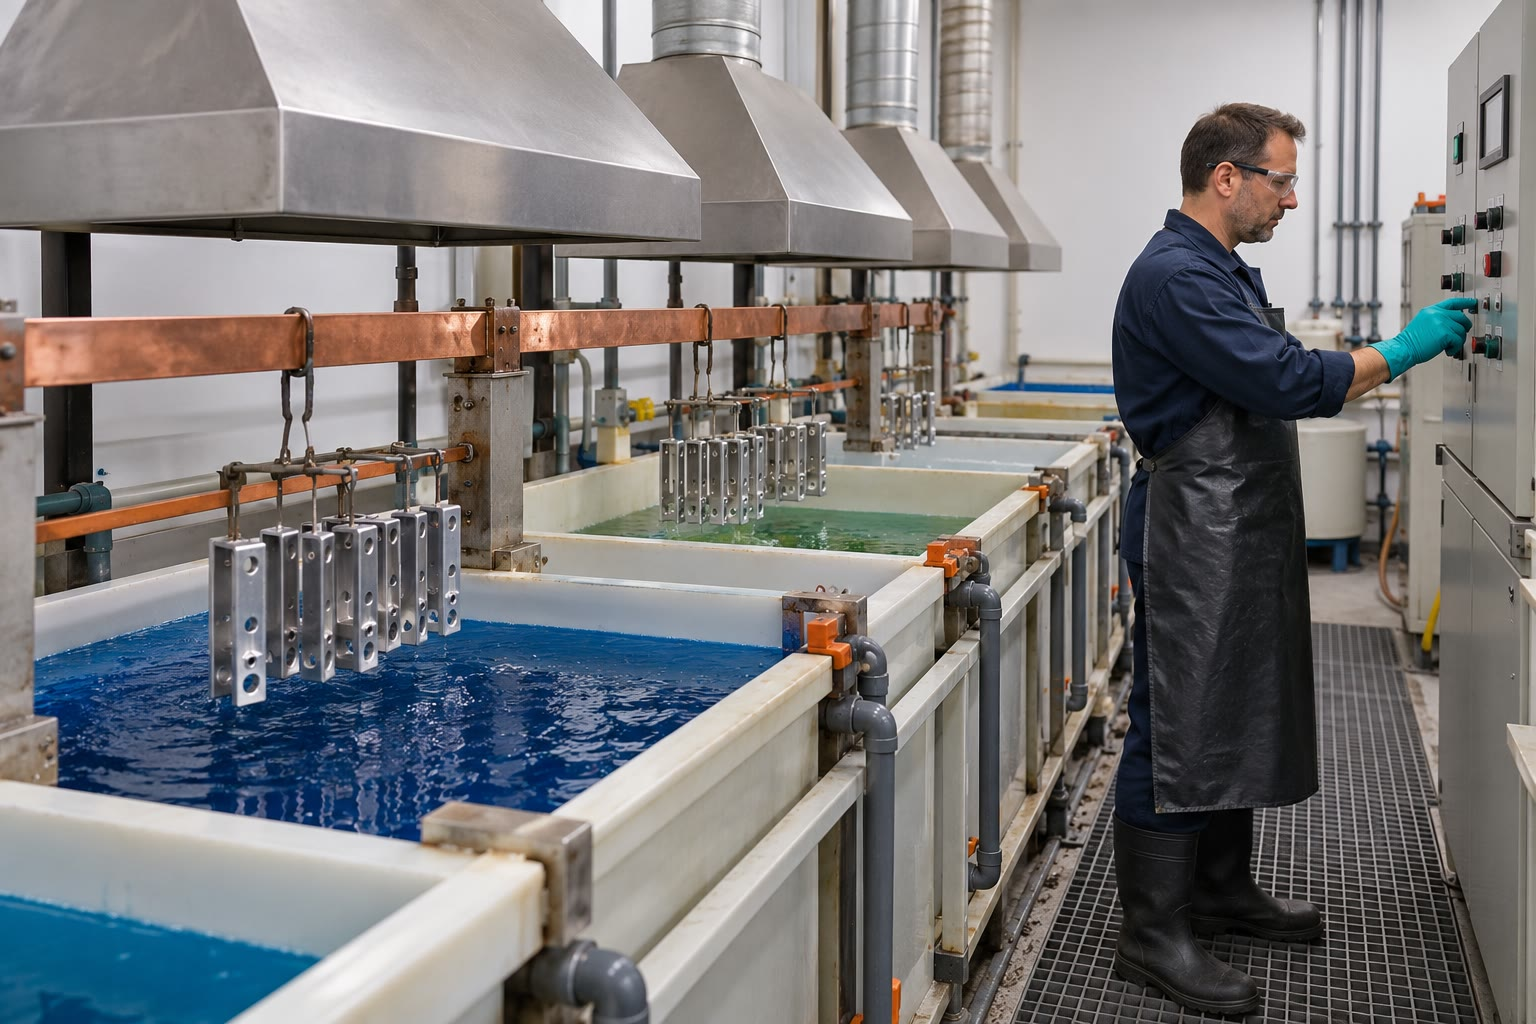
\includegraphics[width=0.62\linewidth]{images/book3/ai/b2-10-electroplating.jpg}

{\small خط طلاء كهربائي: تتدلى القطع المراد طلاؤها من قضبان توزيع نحاسية
في الأحواض وتُجعل مهبطًا؛ ويضبط العامل التيار
عند المقوّم. فالتيار يحدد سرعة ترسب الفلز؛ وجهد
القطع يقرر أي فلز يتكوّن، أو كم من الهيدروجين يتكوّن معه.}
\end{omfigure}

\section{قطب خارج التوازن}

\begin{definition}[منحنى شدة التيار--الجهد]\label{def:b2:current-potential-curves:ie-curve}
\emph{منحنى شدة التيار--الجهد}\index{منحنى شدة التيار--الجهد} لقطب
في محلول هو المنحنى البياني للتيار $i$ المار في القطب
بدلالة جهده $E$. و\emph{التيار المصعدي}\index{تيار مصعدي}،
المعدود موجبًا، يوافق أكسدة عند القطب؛ و\emph{التيار
المهبطي}\index{تيار مهبطي}، المعدود سالبًا، يوافق
اختزالًا.
\end{definition}

\begin{definition}[النوع الكهرنشط]\label{def:b2:current-potential-curves:electroactive}
\emph{النوع الكهرنشط}\index{نوع كهرنشط} نوع كيميائي
يمكن أن يتأكسد أو يُختزل عند القطب في مجال الجهود
المعتبر.
\end{definition}

\begin{proposition}[التيار والسرعة]\label{prop:b2:current-potential-curves:current-rate}
إذا جرى عند قطب نصف تفاعل وحيد مع $n$ إلكترونًا، فإن
التيار يقيس سرعته: $i = nF\,d\xi/dt$، حيث $\xi$ تقدم
الأكسدة (بحيث $i > 0$ لأكسدة، و$i < 0$ لاختزال).
\end{proposition}

\begin{proof}
حسب \cref{prop:b2:cell-thermodynamics:charge}، ينقل التقدم $d\xi$
الشحنة $nF\,d\xi$ عبر القطب في الزمن $dt$.
\end{proof}

لتسجيل منحنى كهذا يجب فرض جهد أحد القطبين
وقياسه بينما يمر فيه تيار --- وهو ما لا تستطيعه خلية ذات قطبين،
لأن التيار يغيّر أيضًا جهد القطب
الثاني.

\begin{definition}[التركيب ذو الأقطاب الثلاثة]\label{def:b2:current-potential-curves:set-up}
في التركيب ذي الأقطاب الثلاثة، يمر التيار بين \emph{القطب
العامل}\index{قطب عامل}، وهو القطب المدروس، و\emph{القطب المساعد}\index{قطب مساعد}،
الذي يغلق الدارة؛ ويُقاس جهد
القطب العامل بالنسبة إلى قطب مرجعي لا يمر فيه
أي تيار. ويضبط مثبِّت جهد إلكتروني التيار بحيث
يحافظ هذا الجهد على القيمة المفروضة.
\end{definition}

\begin{omfigure}
\begin{tikzpicture}[font=\small, >={Stealth}]
  \pic[transform shape] at (0,0) {beaker={0.7}{omDef!14}};
  \pic at (-0.55,0.25) {electrode={black!35}};
  \pic at (0.55,0.25) {electrode={black!15}};
  \pic (r) at (0.0,0.15) {probe};
  \draw[thick, rounded corners] (-2.2,4.3) rectangle (2.2,5.5);
  \node at (0,4.9) {مثبِّت الجهد};
  \draw[thick, omThm] (-0.40,2.65) -- (-0.40,3.5) -- (-1.6,3.5) -- (-1.6,4.3);
  \draw[thick, omDef] (0.70,2.65) -- (0.70,3.5) -- (1.6,3.5) -- (1.6,4.3);
  \draw[thick] (r-top) -- (0,4.3);
  \node[anchor=east, font=\scriptsize, omThm] at (-1.65,3.85) {العامل};
  \node[anchor=west, font=\scriptsize, omDef] at (1.65,3.85) {المساعد};
  \node[anchor=west, font=\scriptsize] at (0.05,3.95) {المرجعي};
  \draw[<-, omProp, thick] (-0.75,1.2) -- (-2.0,1.4) node[left, text=black, align=right] {القطب\\ العامل};
  \draw[<-, omProp, thick] (0.85,1.2) -- (2.1,1.4) node[right, text=black, align=left] {القطب\\ المساعد};
  \draw[<-, omProp, thick] (0.05,0.5) -- (1.4,-0.4) node[right, text=black] {القطب المرجعي};
  \node[font=\scriptsize, align=center] at (0,6.0) {\foreignlanguage{arabic}{يفرض $E_{\text{عامل}} - E_{\text{مرجعي}}$، ويقيس $i$}};
\end{tikzpicture}

{\small التركيب ذو الأقطاب الثلاثة. يدفع مثبِّت الجهد التيار
بين \omterm{def:b2:current-potential-curves:set-up}{القطب العامل} \omterm{def:b2:current-potential-curves:set-up}{والقطب المساعد} بحيث
يُبقي جهد \omterm{def:b2:current-potential-curves:set-up}{القطب العامل}، المقيس بالنسبة إلى القطب
المرجعي، عند القيمة المفروضة؛ ولا يمر أي تيار في
القطب المرجعي.}
\end{omfigure}

حين لا يمر أي تيار وتكون صورتا المزدوجة موجودتين، يأخذ القطب
جهد نرنست للمزدوجة --- إذا كان تبادل الإلكترونات سريعًا بما يكفي
لإقامته. وإبعاد الجهد عنه يجعل تيارًا
يمر.

\section{الأنظمة السريعة والبطيئة}

\begin{definition}[فرط الجهد]\label{def:b2:current-potential-curves:overpotential}
\emph{فرط الجهد}\index{فرط الجهد} لقطب يمر فيه
تيار $i$ هو $\eta = E(i) - E_{\text{توازن}}$، أي الفرق بين
جهده وجهد التوازن (جهد نرنست) للمزدوجة. و\emph{جهد
العتبة}\index{جهد العتبة} لنصف تفاعل هو
الجهد الذي يصير تياره بعده ملحوظًا.
\end{definition}

\begin{definition}[الأنظمة السريعة والبطيئة]\label{def:b2:current-potential-curves:fast-slow}
تكون المزدوجة \emph{نظامًا سريعًا}\index{نظام سريع} على قطب معيّن إذا
مر تيار ملحوظ بمجرد ابتعاد الجهد عن جهد
نرنست لها؛ وتكون \emph{نظامًا بطيئًا}\index{نظام بطيء} إذا لزم \omterm{def:b2:current-potential-curves:overpotential}{فرط جهد}
قدره بضعة أعشار الفولط قبل أن يصير التيار ملحوظًا، في
كلا الاتجاهين.
\end{definition}

كون النظام سريعًا أو بطيئًا يتعلق بالمزدوجة وبمادة
القطب. فالمزدوجتان $\ce{Fe^3+}/\ce{Fe^2+}$ و$\ce{Ag+}/\ce{Ag}$ سريعتان على
البلاتين؛ واختزال \ce{H+} سريع على البلاتين لكنه بطيء على الزئبق
والرصاص والزنك؛ وأكسدة الماء إلى ثنائي الأكسجين بطيئة على كل قطب.
وتبادلات الإلكترونات التي تكسر روابط أو تكوّنها، كتبادلات \ce{O2} أو \ce{H2}،
بطيئة عادة؛ أما نقل إلكترون بين أيونين متقاربي
الشكل فسريع. وشكل الجزء الصاعد من منحنى بطيء يأتي من
حركية نقل الإلكترون، التي يستنتجها مجلد السنة الثالثة.

\begin{omfigure}
\begin{tikzpicture}
\begin{axis}[omie, width=0.47\linewidth, height=5.4cm, xmin=0.25, xmax=1.3,
  ymin=-1.3, ymax=1.3, xlabel={$E$}, ylabel={$i$}, title={\small نظام سريع}]
\addplot[omanodic] table[x=E, y=i, restrict expr to domain={\thisrow{i}}{0:2}] {figdata/out/bachelor-2-ie-curves-a.dat};
\addplot[omcathodic] table[x=E, y=i, restrict expr to domain={\thisrow{i}}{-2:0}] {figdata/out/bachelor-2-ie-curves-a.dat};
\draw[densely dotted] (axis cs:0.77,-1.2) -- (axis cs:0.77,1.2);
\node[font=\scriptsize, anchor=north west] at (axis cs:0.78,-0.05) {$E_{\text{توازن}}$};
\node[font=\scriptsize, anchor=south] at (axis cs:1.1,1.0) {\babelsublr{\ce{Fe^2+} $\to$ \ce{Fe^3+}}};
\node[font=\scriptsize, anchor=north] at (axis cs:0.45,-1.0) {\babelsublr{\ce{Fe^3+} $\to$ \ce{Fe^2+}}};
\end{axis}
\end{tikzpicture}\hfill
\begin{tikzpicture}
\begin{axis}[omie, width=0.47\linewidth, height=5.4cm, xmin=-0.25, xmax=1.8,
  ymin=-1.3, ymax=1.3, xlabel={$E$}, ylabel={$i$}, title={\small نظام بطيء}]
\addplot[omanodic] table[x=E, y=i, restrict expr to domain={\thisrow{i}}{0:2}] {figdata/out/bachelor-2-ie-curves-c.dat};
\addplot[omcathodic] table[x=E, y=i, restrict expr to domain={\thisrow{i}}{-2:0}] {figdata/out/bachelor-2-ie-curves-c.dat};
\draw[densely dotted] (axis cs:0.77,-1.2) -- (axis cs:0.77,1.2);
\draw[<->, omProp] (axis cs:0.77,0.5) -- (axis cs:1.12,0.5) node[midway, above, font=\scriptsize] {$\eta_a$};
\draw[<->, omProp] (axis cs:0.42,-0.5) -- (axis cs:0.77,-0.5) node[midway, below, font=\scriptsize] {$\eta_c$};
\node[font=\scriptsize, anchor=north west] at (axis cs:0.78,-0.05) {$E_{\text{توازن}}$};
\end{axis}
\end{tikzpicture}

{\small منحنيات نموذجية لشدة التيار--الجهد لمزدوجة صورتاها موجودتان
بتركيزين متساويين (الفرع المصعدي بالأحمر، والمهبطي بالأزرق). يمينًا، \omterm{def:b2:current-potential-curves:fast-slow}{نظام
سريع}: يغيّر التيار إشارته بحدة عند جهد التوازن. يسارًا،
\omterm{def:b2:current-potential-curves:fast-slow}{نظام بطيء}: لا يمر أي تيار على مجال من الجهود حوله؛ ويحتاج كل
فرع إلى \omterm{def:b2:current-potential-curves:overpotential}{فرط جهد}. ويبلغ كلاهما الاستواءين الحديين نفسيهما، اللذين يحددهما
الانتشار. (قيم توضيحية.)}
\end{omfigure}

\section{انتقال المادة والتيارات الحدية}

حين يكون نقل الإلكترون سريعًا، يحدّ التيارَ وصولُ
المتفاعل إلى القطب. ففي محلول محرَّك، تبقى طبقة رقيقة من السائل
ملاصقة للقطب ساكنة تقريبًا، ويعبرها المتفاعل
بالانتشار.

\begin{definition}[طبقة الانتشار والتيار الحدي]\label{def:b2:current-potential-curves:limiting-current}
\emph{طبقة الانتشار}\index{طبقة الانتشار} هي طبقة المحلول،
التي سمكها $\delta$ (من بضعة ميكرومترات إلى بضع عشرات منها في محلول
محرَّك)، الملاصقة للقطب، التي لا تتحرك الأنواع عبرها إلا
بالانتشار. و\emph{التيار الحدي}\index{تيار حدي} هو التيار
المبلوغ حين يُستهلك \omterm{def:b2:current-potential-curves:electroactive}{النوع الكهرنشط} بسرعة وصوله، فيكون
تركيزه عند السطح معدومًا.
\end{definition}

\begin{omfigure}
\begin{tikzpicture}[font=\small, >={Stealth}, x=1.2cm, y=1.2cm]
  \fill[black!25] (-0.4,0) rectangle (0,3);
  \node[rotate=90, font=\scriptsize] at (-0.2,1.5) {القطب};
  \draw[->] (0,0) -- (4.6,0) node[right] {$x$};
  \draw[->] (0,0) -- (0,3.2) node[above] {$c$};
  \draw[densely dashed] (1.6,0) -- (1.6,3);
  \node[below, font=\scriptsize] at (1.6,0) {$\delta$};
  \draw[omDef, thick] (0,1.2) -- (1.6,2.4) -- (4.4,2.4);
  \draw[omThm, thick] (0,0.02) -- (1.6,2.4);
  \node[font=\scriptsize, anchor=west] at (2.6,2.6) {\shortstack{\foreignlanguage{arabic}{داخل المحلول، $c^b$ (محرَّك)}}};
  \node[font=\scriptsize, omDef, anchor=east] at (-0.45,1.2) {$c^s$};
  \node[font=\scriptsize, omThm, anchor=west] at (1.7,0.5) {\foreignlanguage{arabic}{$c^s = 0$: تيار حدي}};
  \node[font=\scriptsize, align=center] at (0.8,3.0) {طبقة\\ الانتشار};
\end{tikzpicture}

{\small تركيز المتفاعل قرب قطب في محلول
محرَّك. يكون التوزع خطيًا عبر \omterm{def:b2:current-potential-curves:limiting-current}{طبقة الانتشار}؛ ويتناسب التدفق، ومن ثم
التيار، مع $c^b - c^s$. ويكون أكبر ما يمكن حين يُستهلك المتفاعل
بمجرد وصوله ($c^s = 0$، بالأحمر).}
\end{omfigure}

\begin{theorem}[التيار الحدي]\label{thm:b2:current-potential-curves:limiting}
من أجل نوع تركيزه في داخل المحلول $c$ ومعامل انتشاره $D$،
يعبر طبقة انتشار سمكها $\delta$ نحو قطب مساحته $A$،
يكون \omterm{def:b2:current-potential-curves:limiting-current}{التيار الحدي}، بالقيمة المطلقة،
\[
  |i_{\lim}| = \frac{nFADc}{\delta} .
\]
\end{theorem}

\begin{proof}
في الحالة المستقرة يكون توزع التركيز في الطبقة خطيًا (فقانون فيك
الثاني مع $\partial c/\partial t = 0$ يعطي $d^2c/dx^2 = 0$)، فيكون التدفق
نحو القطب $j = D(c - c^s)/\delta$، بالمول لكل وحدة مساحة ووحدة
زمن. وكل جزيء يصل يتفاعل مع $n$ إلكترونًا: $|i| = nFAj =
nFAD(c - c^s)/\delta$، وهو أكبر ما يمكن من أجل $c^s = 0$.
\end{proof}

\begin{example}[رتبة قدر تيار حدي]\label{ex:b2:current-potential-curves:ilim}
من أجل نوع تركيزه \qty{10}{mmol/L} (\qty{10}{mol/m^3})، مع $D =
\qty{7e-10}{m^2/s}$، و$\delta = \qty{20}{\micro m}$، و$n = 1$، على
\qty{1.0}{cm^2}: $|i_{\lim}| = 96\,485 \times 10^{-4} \times 7 \times 10^{-10}
\times 10/(2 \times 10^{-5}) = \qty{3.4}{mA}$.
\end{example}

\begin{theorem}[موجة نظام سريع]\label{thm:b2:current-potential-curves:wave}
من أجل مزدوجة سريعة $\mathrm{Ox} + n\,\mathrm e^- \rightleftharpoons \mathrm{Red}$،
تيارها الحدي المصعدي $i_{\lim,a} > 0$ (يحدده Red) وتيارها الحدي
المهبطي $i_{\lim,c} < 0$ (يحدده Ox)، يكون المنحنى في الحالة المستقرة
\[
  E = E_{1/2} + \frac{RT}{nF}\ln\frac{i - i_{\lim,c}}{i_{\lim,a} - i},
  \qquad E_{1/2} = E^\circ + \frac{RT}{nF}\ln\frac{D_{\text{Red}}}{D_{\text{Ox}}} ,
\]
مع افتراض سمك الطبقة نفسه للصورتين.
\end{theorem}

\begin{proof}
\omterm{def:b2:current-potential-curves:fast-slow}{نظام سريع}: تصح معادلة نرنست عند السطح، $E = E^\circ + (RT/nF)
\ln(c^s_{\text{Ox}}/c^s_{\text{Red}})$. وتوزعات خطية: \omterm{def:b2:current-potential-curves:ie-curve}{التيار المصعدي} $i$
يستهلك Red وينتج Ox عند السطح، $i = nFAD_{\text{Red}}(c^b_{\text{Red}}
- c^s_{\text{Red}})/\delta = -nFAD_{\text{Ox}}(c^b_{\text{Ox}} - c^s_{\text{Ox}})/\delta$.
ومع $i_{\lim,a} = nFAD_{\text{Red}}c^b_{\text{Red}}/\delta$ و$i_{\lim,c} =
-nFAD_{\text{Ox}}c^b_{\text{Ox}}/\delta$، نحصل على $c^s_{\text{Red}} = (i_{\lim,a} -
i)\delta/(nFAD_{\text{Red}})$ و$c^s_{\text{Ox}} = (i - i_{\lim,c})\delta/(nFAD_{\text{Ox}})$.
نعوّض في معادلة نرنست.
\end{proof}

\begin{corollary}[جهد نصف الموجة]\label{cor:b2:current-potential-curves:half-wave}
حين يتساوى معاملا انتشار الصورتين، يكون $E_{1/2} = E^\circ$: فمع
وجود صورة واحدة فقط، يساوي التيار نصف قيمته الحدية عند الجهد
المعياري للمزدوجة.
\end{corollary}

\begin{proof}
مع وجود Red وحده، $i_{\lim,c} = 0$، ومن أجل $i = i_{\lim,a}/2$ ينعدم
اللوغاريتم: $E = E_{1/2} = E^\circ$ حين $D_{\text{Red}} = D_{\text{Ox}}$.
\end{proof}

\begin{proposition}[الاستواءات تقيس التراكيز]\label{prop:b2:current-potential-curves:plateau}
عند تحريك وقطب ثابتين، يتناسب ارتفاع الاستواء مع
تركيز النوع الذي يستهلكه: فالقطب المحفوظ عند
جهد على الاستواء مجس أمبيرومتري.
\end{proposition}

\begin{proof}
$|i_{\lim}| = (nFAD/\delta)\,c$ والعامل بين القوسين ثابت عند تحريك
ودرجة حرارة ثابتين.
\end{proof}

\begin{omfigure}
\begin{tikzpicture}
\begin{axis}[omie, width=0.47\linewidth, height=5.0cm, xmin=0.25, xmax=1.3,
  ymin=-0.3, ymax=1.3, xlabel={$E$}, ylabel={$i$}, title={\small \foreignlanguage{arabic}{\ce{Fe^2+} وحده موجود}}]
\addplot[omanodic] table[x=E, y=i] {figdata/out/bachelor-2-ie-curves-b.dat};
\draw[densely dotted] (axis cs:0.77,0) -- (axis cs:0.77,0.5) -- (axis cs:0.25,0.5);
\node[font=\scriptsize, anchor=north] at (axis cs:0.77,-0.02) {$E_{1/2}$};
\node[font=\scriptsize, anchor=south west] at (axis cs:0.27,0.5) {$i_{\lim}/2$};
\node[font=\scriptsize, anchor=south] at (axis cs:1.12,1.0) {استواء};
\end{axis}
\end{tikzpicture}\hfill
\begin{tikzpicture}
\begin{axis}[width=0.42\linewidth, height=5.0cm, xmin=0, xmax=1.05, ymin=0, ymax=1.1,
  axis x line=bottom, axis y line=left, xtick=\empty, ytick=\empty,
  xlabel={$c$}, ylabel={$i_{\lim}$}, label style={font=\small},
  title={\small القياس الأمبيرومتري}]
\addplot[omanodic, mark=*, mark size=1.2pt] table[x=c, y=i] {figdata/out/bachelor-2-ie-curves-e.dat};
\end{axis}
\end{tikzpicture}

{\small يمينًا: موجة مزدوجة سريعة حين لا توجد إلا الصورة المختزلة
(نموذج)؛ ويقع نصف ارتفاعها عند جهد نصف الموجة. يسارًا: يكبر ارتفاع
الاستواء بالتناسب مع التركيز.}
\end{omfigure}

\section{المذيب والقطب}

الماء نفسه كهرنشط: فهو يتأكسد إلى ثنائي الأكسجين
(\ce{2H2O -> O2 + 4H+ + 4e-}) ويُختزل إلى ثنائي الهيدروجين (\ce{2H+ + 2e- -> H2}، أو
\ce{2H2O + 2e- -> H2 + 2OH-}). ولأن المذيب لا ينفد أبدًا، فلا استواء
لمنحنياته: إذ تصعد بحدة وتحدّ كل المنحنيات الأخرى.

\begin{definition}[نافذة الكهرنشاطية]\label{def:b2:current-potential-curves:window}
\emph{جدارا المذيب}\index{جدار المذيب} هما الفرعان الشديدا الانحدار
لأكسدة المذيب واختزاله. و\emph{نافذة
الكهرنشاطية}\index{نافذة الكهرنشاطية} هي مجال الجهود بينهما،
الذي يمكن أن تُرصد فيه منحنيات الأنواع المذابة.
\end{definition}

\begin{proposition}[نافذة الماء]\label{prop:b2:current-potential-curves:window}
في الماء عند pH معيّن تقع النافذة حول المجال الترموديناميكي
لمزدوجتي الماء، $\qty{0}{V} - 0.059\,\mathrm{pH}$ و$\qty{1.23}{V} -
0.059\,\mathrm{pH}$، موسَّعًا من كل جهة \omterm{def:b2:current-potential-curves:overpotential}{بفرط جهد}
التفاعل الموافق على القطب المستعمل.
\end{proposition}

\begin{proof}[تعليل]
يبدأ كل جدار قرب جهد نرنست لمزدوجته منزاحًا بفرط
\omterm{def:b2:current-potential-curves:overpotential}{جهد العتبة}: فأكسدة الماء بطيئة على كل الأقطاب، فيقع
الجدار المصعدي فوق \qty{1.23}{V} ببضعة أعشار الفولط (عند pH 0)؛ أما
اختزال \ce{H+} فسريع على البلاتين، الذي يبقى جداره المهبطي قريبًا من
\qty{0}{V}، لكنه بطيء على الزنك أو الرصاص أو الزئبق، التي يقع جدارها أدنى
بعدة أعشار من الفولط.
\end{proof}

\begin{omfigure}
\begin{tikzpicture}
\begin{axis}[omie, width=0.82\linewidth, height=5.4cm, xmin=-1.2, xmax=2.0,
  ymin=-3, ymax=3, xlabel={\babelsublr{$E$ (V)}}, ylabel={$i$}, clip=true, clip mode=individual]
\addplot[omwall] table[x=E, y=i] {figdata/out/bachelor-2-ie-curves-d-high.dat};
\addplot[omcathodic] table[x=E, y=i, restrict expr to domain={\thisrow{E}}{-1.2:0.6}] {figdata/out/bachelor-2-ie-curves-d-Pt.dat};
\addplot[omanodic] table[x=E, y=i, restrict expr to domain={\thisrow{E}}{0.6:2.0}] {figdata/out/bachelor-2-ie-curves-d-Pt.dat};
\draw[densely dotted] (axis cs:0,-2.8) -- (axis cs:0,2.8);
\draw[densely dotted] (axis cs:1.23,-2.8) -- (axis cs:1.23,2.8);
\node[font=\scriptsize, anchor=north west] at (axis cs:0.02,-0.1) {0};
\node[font=\scriptsize, anchor=north west] at (axis cs:1.24,-0.1) {1.23};
\node[font=\scriptsize, omDef, anchor=west] at (axis cs:0.05,-2.2) {\foreignlanguage{arabic}{\babelsublr{\ce{H+} $\to$ \ce{H2}} على \babelsublr{Pt}}};
\node[font=\scriptsize, gray, anchor=east] at (axis cs:-0.85,-1.0) {\foreignlanguage{arabic}{على \babelsublr{Zn}، \babelsublr{Pb}}};
\node[font=\scriptsize, omThm, anchor=east] at (axis cs:1.18,2.2) {\babelsublr{\ce{H2O} $\to$ \ce{O2}}};
\end{axis}
\end{tikzpicture}

{\small جدارا الماء عند pH 0 (نموذج). يبدأ اختزال \ce{H+} قرب
\qty{0}{V} على البلاتين (بالأزرق) لكنه يبدأ أدنى بعدة أعشار من الفولط على فلزات مثل
الزنك أو الرصاص (المتقطع)؛ وتحتاج أكسدة الماء إلى \omterm{def:b2:current-potential-curves:overpotential}{فرط جهد} على أي
قطب. والنافذة هي المجال الواقع بين الجدارين.}
\end{omfigure}

\section{قراءة المنحنيات}

\begin{method}[رسم منحنيات محلول بخطوط تقريبية]\label{met:b2:current-potential-curves:sketch-ie}
\begin{enumerate}
  \item ارسم جداري المذيب الموافقين لقيمة pH ولمادة
        القطب.
  \item لكل مزدوجة موجودة، ضع جهد نرنست لها (إن وُجدت الصورتان
        معًا) أو $E^\circ$ (إن وُجدت صورة واحدة): \omterm{def:b2:current-potential-curves:fast-slow}{فالنظام السريع} يقطع المحور هناك
        بحدة؛ \omterm{def:b2:current-potential-curves:fast-slow}{والنظام البطيء} ينزاح بفرطي جهده.
  \item أعطِ كل موجة استواءً يتناسب مع تركيز النوع
        الذي تستهلكه؛ والقطب الفلزي الذي يتأكسد هو نفسه لا استواء له
        (فالفلز لا ينفد).
  \item اجمع تيارات التفاعلات الممكنة عند كل جهد.
\end{enumerate}
\end{method}

\begin{method}[قراءة المنحنيات]\label{met:b2:current-potential-curves:read-ie}
\begin{enumerate}
  \item عند جهد مفروض، اقرأ على كل منحنى تيار كل
        تفاعل: فهي تجري معًا، بنسبة تياراتها.
  \item عند تيار مفروض (تحليل كهربائي)، جِد الجهد الذي يكون مجموع
        المنحنيات المصعدية أو المهبطية عنده مساويًا لهذا التيار؛ والتفاعلات
        المعنية هي التي تساهم منحنياتها هناك.
  \item في خلية، أو في فلز يتآكل، يساوي \omterm{def:b2:current-potential-curves:ie-curve}{التيار المصعدي} لأحد التفاعلين
        \omterm{def:b2:current-potential-curves:ie-curve}{التيار المهبطي} للآخر: فابحث عن هذا الزوج من
        النقاط.
\end{enumerate}
\end{method}

\begin{example}[الطلاء بالزنك من حوض حمضي]\label{ex:b2:current-potential-curves:zinc}
في حوض زنك حمضي، يحمل المهبط اختزالين ممكنين: \ce{Zn^2+
+ 2e- -> Zn} ($E^\circ = \qty{-0.76}{V}$، سريع) و\ce{2H+ + 2e- -> H2}
($E^\circ = \qty{0}{V}$). فترموديناميكيًا ينبغي أن يأتي الهيدروجين أولًا وألا يأتي الزنك
أبدًا. لكن اختزال \ce{H+} على الزنك بطيء: فجداره يقع تحت
\qty{-0.76}{V}، وعند الجهد الذي يترسب فيه الزنك بسرعة نافعة
لا يتكوّن إلا قليل من الهيدروجين. فالمنحنى، لا المخطط، هو ما يفسر
الطلاء.
\end{example}

\begin{history}[البولاروغرافيا]
\begin{minipage}[t]{0.25\linewidth}
\vspace{0pt}
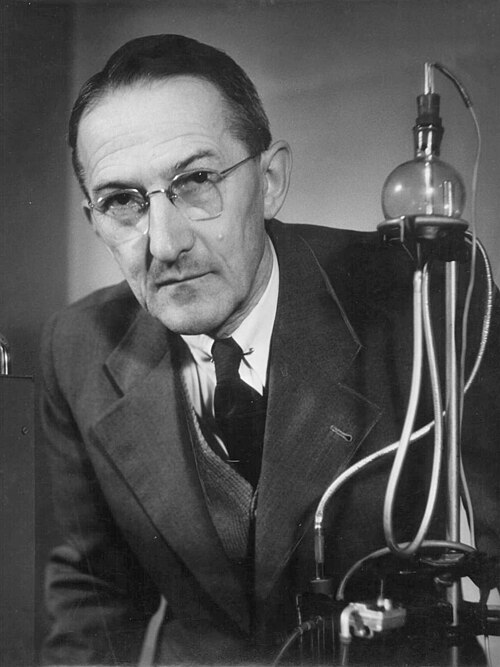
\includegraphics[width=\linewidth]{images/book3/heyrovsky.jpg}
\end{minipage}\hfill
\begin{minipage}[t]{0.71\linewidth}
\vspace{0pt}
سجّل ياروسلاف هايروفسكي سنة 1922 التيار المار في قطب زئبقي
يتكوّن قطرة بعد قطرة عند طرف أنبوب شعري، بينما يُمسح
الجهد: فكل نوع قابل للاختزال يعطي درجة يحدد موقعها هويته
ويقيس ارتفاعها تركيزه. وكانت القطرة المتجددة تُبقي السطح
جديدًا، وفتح \omterm{def:b2:current-potential-curves:overpotential}{فرط جهد} الهيدروجين المرتفع على الزئبق نافذة
مهبطية واسعة. وأكسبته البولاروغرافيا جائزة نوبل في الكيمياء سنة 1959
وأسست الكيمياء التحليلية الكهربائية؛ وتُظهره الصورة مع قطب
الزئبق المتقاطر. (صورة: أرشيف معهد ي.~هايروفسكي
للكيمياء الفيزيائية، CC~BY-SA~3.0، ويكيميديا كومنز.)
\end{minipage}
\end{history}

\section{تمارين}

\begin{exercise}[$\star$]\label{exo:b2:current-potential-curves:1}
في خلية دانييل تعطي تيارًا، أعطِ إشارة التيار عند قطب
الزنك وعند قطب النحاس، وفق اصطلاحات هذا
الفصل.
\end{exercise}

\begin{exercise}[$\star$]\label{exo:b2:current-potential-curves:2}
احسب \omterm{def:b2:current-potential-curves:limiting-current}{التيار الحدي} لاختزال \ce{Ag+} (\qty{2.0}{mmol/L}، $D =
\qty{1.6e-9}{m^2/s}$) على \qty{0.50}{cm^2} مع $\delta = \qty{25}{\micro m}$
(قيم نموذجية).
\end{exercise}

\begin{exercise}[$\star$]\label{exo:b2:current-potential-curves:3}
على المنحنيات النموذجية في الفصل، كيف تتعرف على \omterm{def:b2:current-potential-curves:fast-slow}{نظام سريع} وعلى \omterm{def:b2:current-potential-curves:fast-slow}{نظام بطيء}؟
وأعطِ مثالًا لكل منهما على البلاتين.
\end{exercise}

\begin{exercise}[$\star$]\label{exo:b2:current-potential-curves:4}
محلول لا يحوي إلا \ce{Fe^2+}. عند أي جهد يبلغ تياره المصعدي
نصف استوائه، إذا كانت الصورتان تنتشران بالطريقة نفسها ($E^\circ = \qty{0.77}{V}$)؟
\end{exercise}

\begin{exercise}[$\star\star$]\label{exo:b2:current-potential-curves:5}
يُمسح قطب بلاتيني في محلول من \ce{Fe^3+} و\ce{Cu^2+} (بتركيزين
متساويين، $E^\circ$ = 0.77 و\qty{0.34}{V}) نحو الجهود السالبة. صِف
المنحنى: الموجات، والاستواءات، وارتفاعاتها، والجدار
المهبطي.
\end{exercise}

\begin{exercise}[$\star\star$]\label{exo:b2:current-potential-curves:6}
في محلول \cref{exo:b2:current-potential-curves:5}، يُحفظ جهد
القطب عند \qty{0.50}{V}، ثم عند \qty{0.10}{V}. ماذا يحدث في
كل حالة؟
\end{exercise}

\begin{exercise}[$\star\star$]\label{exo:b2:current-potential-curves:7}
أعطِ جهدي نرنست لمزدوجتي الماء عند pH 0 وعند pH 14، وارسم
بخطوط تقريبية كيف تنتقل النافذة على البلاتين مع قيمة pH.
\end{exercise}

\begin{exercise}[$\star\star$]\label{exo:b2:current-potential-curves:8}
يُعايَر \ce{Fe^2+} بأيونات \ce{Ce^4+} بينما يسجّل قطب بلاتيني محفوظ عند
\qty{1.0}{V} التيار. ارسم بخطوط تقريبية التيار بدلالة الحجم المضاف
وفسّر كيف يحدد موقع التكافؤ ($\ce{Ce^4+}/\ce{Ce^3+}$: $E^\circ =
\qty{1.72}{V}$).
\end{exercise}

\begin{exercise}[$\star\star$]\label{exo:b2:current-potential-curves:9}
مضاعفة سرعة التحريك تنصّف سمك \omterm{def:b2:current-potential-curves:limiting-current}{طبقة الانتشار}. ماذا
يحدث للاستواءات، ولجهد نصف الموجة، ولجهد التيار
المعدوم \omterm{def:b2:current-potential-curves:fast-slow}{لنظام سريع}؟
\end{exercise}

\begin{exercise}[$\star\star\star$]\label{exo:b2:current-potential-curves:10}
استنتج معادلة موجة \omterm{def:b2:current-potential-curves:fast-slow}{نظام سريع} مع وجود Red وحده، 
وبيّن أن رسم $E$ بدلالة $\log[i/(i_{\lim} - i)]$ مستقيم
ميله $0.059/n$ فولط عند \qty{25}{\degreeCelsius}.
\end{exercise}

\begin{exercise}[$\star\star\star$]\label{exo:b2:current-potential-curves:11}
قطعة من الزنك مغموسة في حمض تركيزه \qty{1}{mol/L} لا تذوب إلا ببطء، بينما
القطعة نفسها الملامسة لسلك بلاتيني تذوب بسرعة، مع تصاعد فقاعات الهيدروجين
على البلاتين. فسّر ذلك بمنحنيات شدة التيار--الجهد.
\end{exercise}

\begin{exercise}[$\star\star\star$]\label{exo:b2:current-potential-curves:12}
لأكسدة نوع تقع موجته عند \qty{2.0}{V} عند pH 0، هل تختار
قطبًا بلاتينيًا أم قطبًا ذا \omterm{def:b2:current-potential-curves:overpotential}{فرط جهد} أكسجين مرتفع؟ علّل، واذكر
ما كان سيتكوّن خلاف ذلك.
\end{exercise}

\section{مسألة: مجس أكسجين لنهر}

\begin{problem}[{مسألة نهاية الأسبوع --- مهبط مجس أكسجين
أمبيرومتري، والتيار الحدي عبر غشائه، والمعايرة في ماء
مشبع بالهواء بقانون هنري، ومحتوى نهر من الأكسجين}]
\label{pb:b2:current-potential-curves:1}
لمجس أكسجين أمبيرومتري مهبط من الذهب ومصعد من الفضة في
هلام من كلوريد البوتاسيوم، يفصلهما عن العيّنة غشاء رقيق نفوذ للغاز.
ويُحفظ المهبط عند \qty{-0.60}{V} بالنسبة إلى مصعد الفضة--كلوريد
الفضة. المعطيات عند \qty{25}{\degreeCelsius}: ثابت \omterm{prop:b2:chemical-potential:henry}{قانون هنري}
لثنائي الأكسجين \ce{O2}، $H = \qty{1.3e-5}{mol/(m^3.Pa)}$؛ وضغط بخار الماء
\qty{3.17}{kPa}؛ والأكسجين في الهواء الجاف 20.95~\% حجمًا؛ و$E^\circ(\ce{O2}/\ce{H2O}) =
\qty{1.229}{V}$؛ و$E^\circ(\ce{AgCl}/\ce{Ag}) = \qty{0.222}{V}$. الغشاء (قيم
نموذجية): مساحته \qty{0.10}{cm^2}، وسمكه \qty{25}{\micro m}، ومعامل الانتشار
الفعلي لثنائي الأكسجين \ce{O2} عبره \qty{1.0e-10}{m^2/s}.
% ledger: henry:O2, pvap:H2O.298, air:O2, dfg:Cl-_ao, dfg:AgCl_cr, aw:O

\medskip
\noindent\textbf{الجزء الأول --- المهبط.}
\begin{enumerate}
  \item اكتب معادلة اختزال ثنائي الأكسجين في وسط متعادل.
  \item اكتب التفاعل عند مصعد الفضة، والتفاعل الإجمالي.
  \item احسب جهد نرنست للمزدوجة $\ce{O2}/\ce{H2O}$ عند pH 7 مع
        $p_{\ce{O2}} = \qty{0.21}{bar}$.
  \item عبّر عن جهد المهبط، \qty{-0.60}{V} بالنسبة إلى \babelsublr{Ag/AgCl}، على
        سلم الهيدروجين، مع أخذ نشاطية الكلوريد في الهلام مساوية 1.
  \item لماذا يجب أن يُحفظ المهبط بعيدًا تحت جهد نرنست
        لثنائي الأكسجين \ce{O2}؟
  \item لماذا يُختار جهد يقع على الاستواء؟
  \item ما الذي يحدد الحد الأدنى للجهود القابلة للاستعمال؟
\end{enumerate}

\medskip
\noindent\textbf{الجزء الثاني --- \omterm{def:b2:current-potential-curves:limiting-current}{التيار الحدي}.}
\begin{enumerate}[resume]
  \item صِف توزع تركيز \ce{O2} عبر الغشاء حين يعمل
        المهبط على استوائه.
  \item اكتب تدفق \ce{O2} عبر الغشاء.
  \item استنتج التيار بدلالة التركيز $c$ لثنائي الأكسجين
        \ce{O2} المذاب.
  \item لماذا يُستعمل سمك الغشاء مكان \omterm{def:b2:current-potential-curves:limiting-current}{طبقة الانتشار}؟
  \item لماذا لا تتعلق القراءة كثيرًا بتحريك ماء النهر، لكنها
        تتعلق كثيرًا باتساخ الغشاء؟
\end{enumerate}

\medskip
\noindent\textbf{الجزء الثالث --- المعايرة.}
\begin{enumerate}[resume]
  \item احسب الضغط الجزئي لثنائي الأكسجين \ce{O2} فوق ماء مشبع بالهواء عند
        \qty{1.013}{bar} و\qty{25}{\degreeCelsius}.
  \item احسب تركيز \ce{O2} المذاب عند الإشباع، بوحدة
        \unit{mol/m^3}.
  \item عبّر عنه بوحدة \unit{mg/L}.
  \item تنبأ بتيار المجس في ماء مشبع بالهواء.
  \item يقرأ المجس فعلًا \qty{4.05}{\micro A} في ماء مشبع بالهواء
        (معطيات تمرين). احسب حساسيته بوحدة \unit{\micro A} لكل
        \unit{mg/L}.
  \item لماذا نعاير بدل أن نثق بالتيار المتنبأ به؟
  \item ماذا ينبغي أن يقرأ المجس في ماء خالٍ من الأكسجين؟
\end{enumerate}

\medskip
\noindent\textbf{الجزء الرابع --- النهر.}
\begin{enumerate}[resume]
  \item في عيّنة من النهر عند \qty{25}{\degreeCelsius}، يقرأ المجس
        \qty{2.80}{\micro A}. احسب الأكسجين المذاب بوحدة \unit{mg/L}.
  \item عبّر عنه نسبةً مئوية من الإشباع.
  \item يكاد ماء النهر يكون مشبعًا بالأكسجين عند منبعه.
        اقترح سببًا للعجز.
  \item ما كمية \ce{O2} التي يستهلكها المجس في ساعة واحدة؟ وهل
        يُخل بالعيّنة؟
  \item لماذا يجب إعادة المعايرة إذا كان النهر عند
        \qty{15}{\degreeCelsius}؟
  \item اذكر تركيز الأكسجين المذاب في العيّنة.
\end{enumerate}
\end{problem}
